\begin{pastexam}[label={px:ntut-112-prog-01}]{北科大資工所 112 學年度 第 1 題}
（程式填空）

\textbf{Problem 1 [12\%] [each 2\%]}

Suppose that the outputs of the following C program are as follows:\\
\hspace*{1em}\texttt{2 3 12 21 23 43 65}

Please trace the program and fill the blanks with correct statements.
\begin{minted}[fontsize=\small, breaklines]{c}
#include <stdio.h>
#include <stdlib.h>
typedef struct node {
      int data;
      struct node *left;
      struct node *right;
} node_t;
typedef node_t * nodep_t;

nodep_t createNode(int value) {
      nodep_t p = (nodep_t) malloc(sizeof(node_t));
      p->data = value;
      p->left = p->right = ________;                /* Problem 1-1 */
      return p;
}
void build(nodep_t current, nodep_t newNode, int value) {
      nodep_t parent;
      while(1) {
            parent = current;
            if(value < parent->data) {
                  current = current->left;
                  if(current == NULL) {
                        ________ = newNode;          /* Problem 1-2 */
                        return;
                  }
            }
            else {
                  current = current->right;
                  if(current == NULL) {
                        ________ = newNode;          /* Problem 1-3 */
                        return;
                  }
            }
      }
}
nodep_t insert(int value, nodep_t root) {
      nodep_t current, parent, newNode;
      newNode = createNode(value);
      if(root == NULL) {
            root = newNode;
      }
else {
            parent = current = ________;             /* Problem 1-4 */
            build(current, newNode, value);
      }
      return root;
}
void inorder_traversal(nodep_t root) {
      if(root != NULL) {
            inorder_traversal(________);             /* Problem 1-5 */
            printf("%d ",root->data);
            inorder_traversal(________);             /* Problem 1-6*/
      }
}
int main() {
      nodep_t root = NULL;
      int array[] = {23,12,43,21,65,3,2};
      for(int i = 0; i < 7; i++)
            root=insert(array[i], root);
      inorder_traversal(root);
      return 0;
}
\end{minted}
\begin{center}
\begin{tabular}{|c|p{6cm}|}
\hline
Problem & \multicolumn{1}{c|}{Answer} \\ \hline
1-1 & \\ \hline 1-2 & \\ \hline 1-3 & \\ \hline 1-4 & \\ \hline 1-5 & \\ \hline 1-6 & \\ \hline
\end{tabular}
\end{center}
Please copy the above answer table to your answer sheet.
\end{pastexam}

\begin{pastsoln}
答案：1-1 \texttt{NULL}；1-2 \texttt{parent->left}；1-3 \texttt{parent->right}；1-4 \texttt{root}；
1-5 \texttt{root->left}；1-6 \texttt{root->right}。

程式是二元搜尋樹的插入（資結書第~9.2~節、虛擬碼~9.6）加中序走訪（資結書第~7.3~節）。 輸出
\texttt{2 3 12 21 23 43 65} 正好是七個數由小到大，這就是二元搜尋樹中序走訪的性質，可以拿來確認空格的方向。

\begin{itemize}
\item \textbf{1-1}：新節點還沒有子節點，左右指標都設成空指標 \texttt{NULL}。 後面 \texttt{build} 用
\texttt{current == NULL} 判斷走到底、\texttt{inorder\_traversal} 用 \texttt{root != NULL} 判斷停止，都靠這個值。
\item \textbf{1-2、1-3}：\texttt{build} 從根往下走，每一步先記住 \texttt{parent = current}，再依 \texttt{value} 和
\texttt{parent->data} 的大小往左或往右走。 \texttt{current} 變成 \texttt{NULL} 時，表示新節點應該接在
\texttt{parent} 的那一邊：往左走到空的就 \texttt{parent->left = newNode}，往右走到空的就
\texttt{parent->right = newNode}。 寫成 \texttt{current = newNode} 不行，那只改了區域變數，樹沒有接上。
\item \textbf{1-4}：樹不是空的時候，從根開始找插入位置，\texttt{parent = current = root}。
\item \textbf{1-5、1-6}：中序是「左子樹、根、右子樹」，\texttt{printf} 夾在中間，前後分別遞迴
\texttt{root->left}、\texttt{root->right}。 如果兩個對調，印出的是由大到小，和題目的輸出不符。
\end{itemize}

\textbf{追蹤。} 依序插入 $23, 12, 43, 21, 65, 3, 2$：$23$ 當根；$12 < 23$ 接在左邊；$43 > 23$ 接在右邊；$21 < 23$、
$21 > 12$，接在 $12$ 的右邊；$65$ 一路往右接在 $43$ 的右邊；$3$ 往左兩次接在 $12$ 的左邊；$2$ 再往左接在 $3$ 的左邊。
\begin{center}
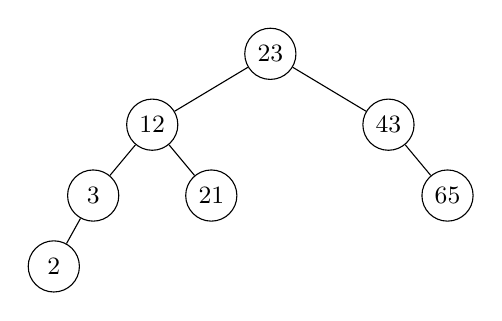
\begin{tikzpicture}[v/.style={circle,draw,minimum size=6.5mm,inner sep=0pt,font=\small},
  level distance=9mm, level 1/.style={sibling distance=30mm}, level 2/.style={sibling distance=15mm},
  level 3/.style={sibling distance=10mm}]
\node[v] {23}
  child {node[v] {12}
    child {node[v] {3} child {node[v] {2}} child[missing]}
    child {node[v] {21}}}
  child {node[v] {43}
    child[missing]
    child {node[v] {65}}};
\end{tikzpicture}
\end{center}
中序走訪：$12$ 的左子樹 $2, 3$，再 $12$、$21$，然後根 $23$，最後右子樹 $43, 65$，得
\texttt{2 3 12 21 23 43 65}，和題目一致。 \texttt{main} 每次用 \texttt{root = insert(...)} 接回傳值，第一次插入時
\texttt{root} 從 \texttt{NULL} 變成新節點，之後回傳的都是原來的根。

補充：\texttt{insert} 裡的區域變數 \texttt{parent} 設了值卻沒用到（真正用的是 \texttt{build} 自己的
\texttt{parent}），不影響結果。 插入一個數的時間和樹高成正比，$O(h)$；這組資料樹高 $4$（以節點數計）。
\end{pastsoln}
